\begin{figure}
    \centering
    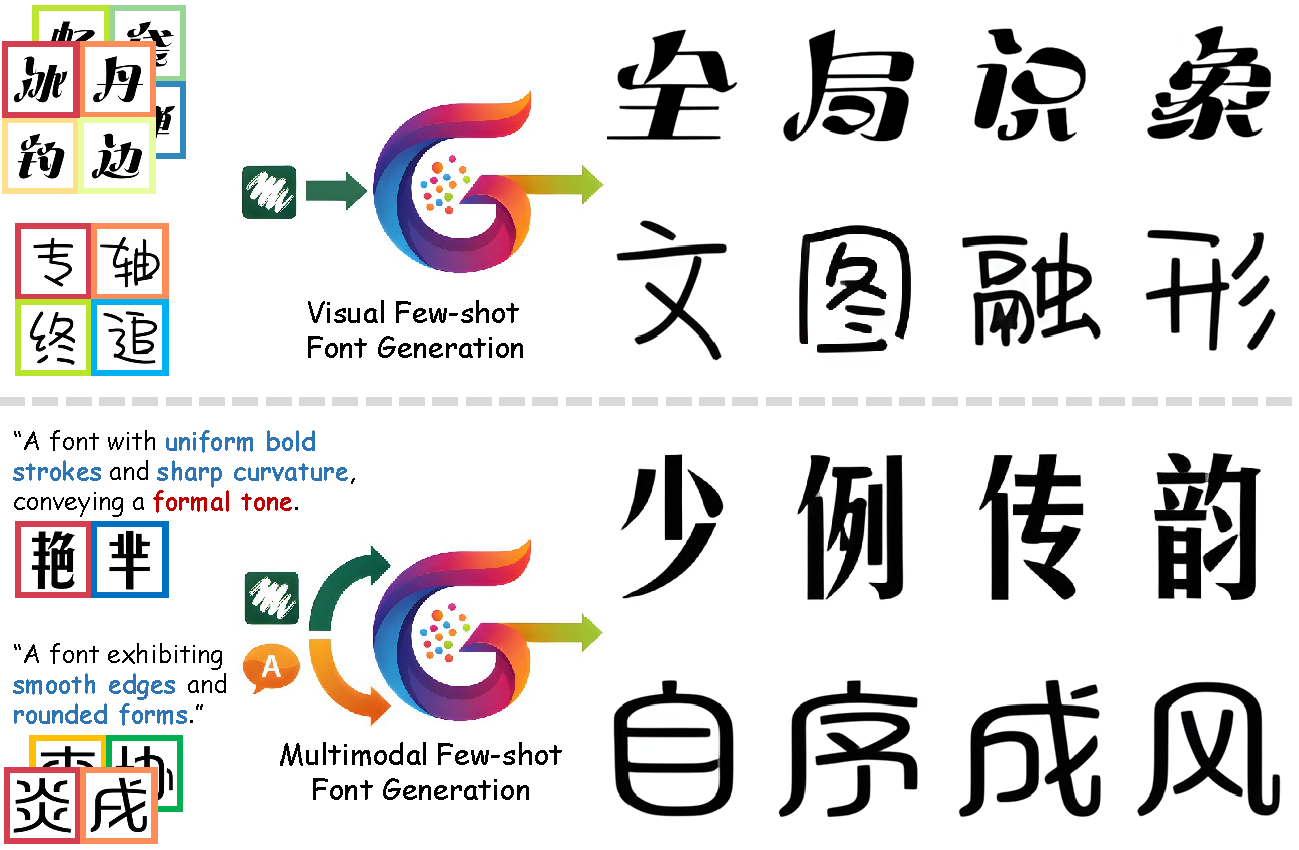
\includegraphics[width=\linewidth]{IMGS/Teaser.pdf}
    \vspace{-3mm}
    \caption{GAR-Font results under visual and multimodal few-shot settings. The generated poem reflects the key contributions of our model: global-aware tokenization for style fidelity, multimodal style encoding for text-image control, reduced reference requirements, and an autoregressive design that enables controllable high-quality font synthesis.}
    \label{fig: Teaser}
    \vspace{-3mm}
\end{figure}
\section{Introduction}

High-quality fonts are central to visual communication, yet their manual creation is costly: practitioners must translate their design concepts into a full, consistent glyph set. This challenge is compounded for logographic systems like Chinese and Japanese, which contain tens of thousands of characters and complex stroke geometries.

Few-shot Font Generation (FFG) seeks to automate this process by generating an entire font library from only a handful of reference examples. However, it presents several technical difficulties. First, it demands precise structural fidelity, where strokes, radicals, and local geometry must be correct for every glyph. Second, it requires capturing a holistic and faithful style representation, generalizing from a handful of examples across diverse characters.

A core obstacle for FFG is the lack of an effective visual global representation. GAN-based methods~\cite{LF_Font, CG_GAN} often exhibit noticeable style discrepancies from the reference fonts, and struggle with stroke-level accuracy. Diffusion models~\cite{Diff_Font, Font_Diffuser, HFH_Font} improve structural correctness and local fidelity but do not guarantee a coherent global style. Existing sequence approaches such as VQ-Font~\cite{VQ_Font} and IF-Font~\cite{IF_Font} rely on local patch or block tokenization, which fragments global cues and leads to noticeable discrepancies from the reference styles. Recent autoregressive (AR) image generation methods~\cite{Titok, SpectralAR} further reveal the superiority of globally contextualized 1D tokens over 2D patched tokenization, highlighting a promising direction for modeling global stylistic patterns in font synthesis. 


Meanwhile, existing FFG frameworks remain single-modal, using only visual modality to control font style. In contrast, linguistic descriptions convey global, conceptual design intents that go beyond visual appearance. They provide complementary representations, helping overcome the limitations of vision-only models when style must be inferred from a few examples.


These insights motivate GAR-Font, an expressive and controllable FFG framework that integrates visual and linguistic information. Leveraging the AR modeling capacity, GAR-Font introduces three major technical contributions:

\begin{itemize}
\item We propose \textbf{a global-aware tokenizer (G-Tok)} that fuses local features with global perception, capturing both fine-grained stroke details and font-level style patterns.
\item We design \textbf{an AR generator with multimodal style encoder}, first pretrained on visual inputs, and then augmented with a lightweight language-style adapter.
\item We introduce \textbf{a post-refinement pipeline} to the font generation process, which improves structural fidelity and stylistic coherence, producing high-quality glyphs from limited references.
\end{itemize}

To validate the effectiveness of GAR-Font, we conduct extensive experiments across multiple settings. In the standard vision-only scenario, it surpasses other competitive FFG methods, demonstrating superior structural and stylistic fidelity. In the multimodal setting, the augmented multimodal style encoder further improves generation quality. Using 4 reference images plus one textual description, GAR-Font matches the quantitative performance of 8 images while providing flexible control. Ablation studies further confirm that G-Tok produces stable and coherent representations that preserve holistic structure and reference style fidelity—key factors for high-quality font synthesis. GAR-Font moves beyond patch-level modeling by learning global-aware representations and enabling text-driven multimodal FFG, establishing a new AR-based solution for automatic and controllable font generation.

% To validate the superiority of GAR-Font, we conduct comprehensive experiments. We compare our method with existing cutting-edge FFG methods in the conventional vision-only scenario, showing its competitive performance. The proposed lightweight language-style adapter further enhances GAR-Font by enabling flexible text-guided style control, improving generation quality while reducing reliance on style references. Moreover, extensive analyses verify the strong global-aware representation capability of the G-Tok, highlighting its ability to preserve holistic structure and coherent style which are key factors for achieving consistent and high-fidelity font synthesis.